\usection{Metodología de Desarrollo Utilizada}

Dado que al inicio del proyecto no se contaba con una definición completa de los requisitos, se necesitaba una metodología que fuera flexible y evolutiva. La elección del modelo de desarrollo se basó en la necesidad de gestionar activamente los riesgos técnicos, permitir una mejora continua a través de iteraciones y adaptar el sistema a los desafíos que surgieran durante la implementación.

\begin{table}[ht]
  \doublespacing
  \centering
  \small
  \begin{tabular}{ c c c c c }
    \hline
    Metodologías & Flexible & Evolutivo & Gestión de riesgos & Iteración y mejora continua \\
    \hline
    Espiral      & Sí       & Sí        & Sí                 & Sí                          \\
    Cascada      & No       & No        & No                 & No                          \\
    Incremental  & No       & Sí        & No                 & Sí                          \\
    Scrum        & Sí       & Sí        & Si                 & Sí                          \\
    \hline
  \end{tabular}
  \caption{Cuadro Comparativo de metodologías}
  \label{tab:comparative-methodologies}
\end{table}

Esto implicaba ciclos de retroalimentación constantes, validación continua y refinamiento iterativo del sistema, características esenciales para alcanzar una solución en un contexto tan dinámico. La elección de una metodología de desarrollo adaptable permitió no solo enfrentar la incertidumbre técnica, sino también ajustar oportunamente el diseño según los aprendizajes obtenidos en cada etapa del proceso. Con esto en mente comparamos las distintas metodologías basándonos en esas necesidades en la Tabla \ref{tab:comparative-methodologies}.

Aunque metodologías ágiles como Scrum también cumplen con estos criterios, se optó por el modelo Espiral debido a su énfasis explícito en el 'Análisis de Riesgos' como una fase formal en cada ciclo. Dada la incertidumbre técnica del proyecto, esta característica fue considerada fundamental para mitigar de manera proactiva cualquier desafío técnico o de gestión que pudiera surgir.

Según lo propuesto por \citeauthor{boehm_spiral_1988} \citeyear{boehm_spiral_1988}, es un enfoque iterativo y flexible que combina elementos del desarrollo incremental y el prototipado, permitiendo gestionar riesgos y adaptar el sistema a medida que avanza el proyecto. Este modelo ha sido ampliamente reconocido por su capacidad para gestionar el desarrollo de sistemas complejos, ya que combina la naturaleza iterativa del prototipado con la estructura sistemática del modelo en cascada \cite[p. 39]{pressman_ingenieria_2010}. En cada iteración, se pueden realizar ajustes en el plan del proyecto, permitiendo adaptar el software a las necesidades emergentes y reducir riesgos antes de que se conviertan en problemas críticos \cite[p. 40]{pressman_ingenieria_2010}.

Según \citeauthor{boehm_spiral_1988} \citeyear{boehm_spiral_1988}, el Modelo Espiral se caracteriza por su estructura cíclica, en la que cada iteración incluye cuatro fases principales:

\begin{enumerate}
  \item \textbf{Determinación de objetivos.} Inicialmente se definen los objetivos específicos de la iteración, identificando las limitaciones del proceso y del sistema de software. Se evalúan alternativas y se especifican condiciones como lenguaje, entornos, entre otros.
  \item \textbf{Análisis de riesgos.} Se identifican y evalúan los riesgos potenciales. Se definen acciones para reducir los riesgos identificados y se evalúan alternativas existentes partiendo de prototipos, simulaciones y softwares de análisis. En este ciclo, existen varios prototipos como plantillas de diseño o componentes funcionales.
  \item \textbf{Desarrollo.} Los prototipos se amplían y se añaden funcionalidades. El código es escrito, probado y migrado a un entorno de prueba varias veces hasta que pueda ser implementado correctamente.
  \item \textbf{Planificación.} Al final de cada iteración se procede a planificar la siguiente, de ser necesaria. Si se producen errores, se buscan soluciones, y si se consiguen mejores alternativas, se implementa en el siguiente ciclo.
\end{enumerate}

Como señala \citeauthor{boehm_spiral_1988} \citeyear{boehm_spiral_1988}, ``el Modelo Espiral es particularmente adecuado para proyectos con altos niveles de incertidumbre y requisitos cambiantes, ya que permite incorporar retroalimentación continua y adaptar el diseño en función de los resultados obtenidos”. En este trabajo, esta metodología permitió gestionar los riesgos técnicos y asegurar que el sistema cumpliera con los objetivos planteados. La Figura \ref{fig:modelo_espiral} ilustra el modelo de desarrollo en espiral propuesto por Boehm (1988).

      \begin{figure}[H]
            \centering
            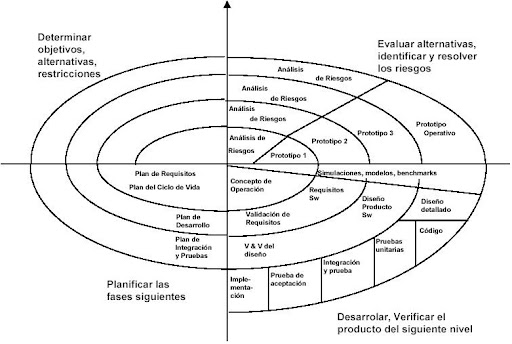
\includegraphics[width=0.85\textwidth]{Anexos/metodologia_espiral.png}
            \caption{Modelo de desarrollo en espiral propuesto por Boehm (1988).}
            \label{fig:modelo_espiral}
      \end{figure}

  % {\small
  %   \begin{longtable}[c]{c p{5.8cm} >{\centering\arraybackslash}p{2cm} p{5.8cm}}
  %     \toprule
  %     ID   & \centering Riesgo                                                                                                                                                                                                                                                 & Probabilidad / Impacto & Estrategia de Mitigación y Monitoreo                                                                                                                                                                                                                                                                                                                                                                                                                       \\
  %     \midrule
  %     \endfirsthead
  %     \toprule
  %     ID   & \centering Riesgo                                                                                                                                                                                                                                                 & Probabilidad / Impacto & Estrategia de Mitigación y Monitoreo                                                                                                                                                                                                                                                                                                                                                                                                                       \\
  %     \midrule
  %     \endhead
  %     \endfoot
  %     \endlastfoot

  %     R-01 & Rendimiento insuficiente del hardware: Que el dispositivo de borde (Edge device)  seleccionado no sea capaz de ejecutar los modelos de IA en tiempo real, generando una latencia inaceptable.                                                        & Alta / Alto            & La estrategia se basa en diseñar una arquitectura modular y distribuida que delegue las tareas computacionalmente pesadas (como el reentrenamiento de modelos) a un servidor local. Paralelamente, se monitorea de forma continua el consumo de CPU y memoria en el dispositivo de borde durante las pruebas para identificar cuellos de botella y optimizar el rendimiento de la inferencia en tiempo real.                                               \\
  %     \addlinespace
  %     R-02 & Abandono por Complejidad de Interacción: Que el usuario final, especialmente si no es técnico, perciba el sistema como una carga y deje de usarlo debido a la necesidad de una interacción o mantenimiento constantes.                                            & Alta / Alto            & Diseñar el sistema bajo el principio de ``cero mantenimiento'' para el usuario. Una vez configurado inicialmente, la única interacción requerida es la respuesta verbal a las consultas del sistema, eliminando la necesidad de gestionar menús, aplicaciones o configuraciones complejas en el día a día.                                                                                                                                                  \\
  %     \addlinespace
  %     R-03 & Baja Precisión (Falsos Positivos/Negativos): Que el sistema genere un alto número de falsos positivos (alertas innecesarias que causan desconfianza) o falsos negativos (fallar en detectar una emergencia real), haciendo que el sistema sea ineficaz o molesto. & Media / Alto           & Implementar un mecanismo de consulta como un segundo filtro para validar si realmente es necesaria una alerta y asi reducir las falsas alarmas.                                                                                                                                                                                                                                                                                                            \\
  %     \addlinespace
  %     R-04 & Fallo en el Canal de Notificación: Que el sistema no pueda enviar una alerta crítica porque el servicio externo del que depende (ej. API de mensajería, servicio de email) falle, cambie sus condiciones o sea descontinuado, dejando al usuario sin aviso.       & Media / Alto           & Diseñar el módulo de notificaciones de forma desacoplada y genérica. Esto permite integrar fácilmente múltiples canales de alerta (ej. email, SMS, Telegram, e incluso dispositivos locales como una sirena o luz inteligente)                                                                                                                                                                                                                             \\
  %     \addlinespace
  %     R-05 & Percepción de Invasión a la Privacidad: Que el usuario o sus visitantes rechacen el sistema por temor a que un micrófono esté ``escuchando'' y enviando conversaciones privadas a la nube, independientemente de las garantías técnicas.                          & Alta / Alto            & Diseñar el sistema bajo el principio de ``Privacidad por Diseño'', asegurando que todo el procesamiento de audio se realice 100\% de forma local en el dispositivo (Edge AI). La arquitectura es modular, separando el sistema de análisis (que opera sin conexión) del módulo de notificaciones. La conexión a internet se utiliza única y exclusivamente para enviar la alerta final (un paquete de datos, no audio), minimizando la exposición a la red. \\
  %     \bottomrule
  %     \addlinespace

  %     \caption{Tabla de Gestión de Riesgos}
  %     \label{tab:risk-management}
  %   \end{longtable}
  % }